\chapter{\IfLanguageName{dutch}{Stand van zaken}{State of the art}}%
\label{ch:stand-van-zaken}

De orderverwerking binnen 3D-printproductie is een proces dat bijdraagt aan de efficiëntie en consistentie van productie. Kleinschalige e-\-commerce bedrijven werken vaak met handmatige methoden voor het verwerken van orders, zoals het controleren of er  nieuwe bestellingen zijn binnengekomen en vervolgens te verwerken, zodat de printer kan starten. Vaak worden er ook Excel-bestanden gebruikt om orders bij te houden, wat tijdrovend en foutgevoelig kan zijn. Door de voortdurende ontwikkeling van technologie is het automatiseren van deze processen interessant. Zo kan er een proces worden opgezet dat dit met behulp van een Pipeline met API-integraties regelt. Dit vermindert fouten en versnelt de bedrijfsvoering. 

\section{Vergelijkbare studies}%
\label{sec:Vergelijkbare studie}

Er zijn al een aantal verschillende vergelijkbare studies die zich richten op de automatisering van productie binnen 3D-printen. In een onderzoek van Maarten van Welsem bespreekt hij wat de impact is van 3D-printtechnologieën op de supply chain. Het beschrijft hoe automatisering een grotere flexibiliteit kan bieden, vooral voor reserveonderdelen en ondemand productie~\autocite{emerce3DprintSupplyChain}. Verder wordt er in een artikel van 3D Print Magazine beschreven hoe de automatisering binnen Europese 3D-printbedrijven hen helpt om mee te kunnen met andere bedrijven, door efficiënt aan de slag te gaan met complexe productieschema's. Ze hebben een grootschalig bedrijf en werken maar met 12 personen om al die printers te besturen door de automatisatie~\autocite{3dprintmagAutomation}. 

\newpage

\section{3D-printen \& industrie}%
\label{sec:3D-printen & industrie}

\subsection{Inleiding}
3D-printen, ook wel bekend als Additive Manufacturing (AM), is een technologie die in de afgelopen decennia een enorme ontwikkeling heeft doorgemaakt \autocite{3dPrintingIndustry}. Deze techniek maakt het mogelijk om driedimensionale objecten laag voor laag op te bouwen met behulp van verschillende materialen zoals plastic, metaal en hars. In deze studie bespreken we de werking van 3D-printen, de industrie, en de Bambu Lab X1C-Carbon als specifieke use case.

\subsection{Wat is 3D-Printen?}
3D-printen is een proces waarbij digitale 3D-modellen worden omgezet in fysieke objecten door opeenvolgende lagen materiaal neer te leggen. Dit proces verschilt van traditionele subtractieve productietechnieken zoals frezen en snijden, omdat het materiaal alleen wordt toegevoegd waar nodig \autocite{3dPrintingIndustry}. Er zijn verschillende 3D-printtechnieken zoals:
\\
\begin{wrapfigure}{r}{0.3\textwidth} % Verklein de breedte van de afbeelding
    \centering
    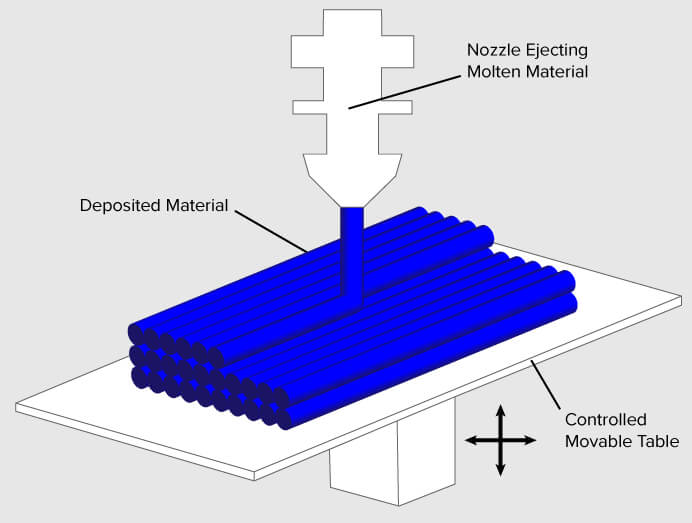
\includegraphics[width=0.8\linewidth]{Foto's/FDM}
    \caption{FDM printtechniek. Bron: \url{https://nederland.3dprinting.com/wat-is-3d-printing/}}
    \label{fig:fdm}
\end{wrapfigure}
\begin{itemize}
    \item Fused Deposition Modeling (FDM)
    \item Stereolithografie (SLA)
    \item Selective Laser Sintering (SLS)
    \item Digital Light Processing (DLP)
\end{itemize}
Voor dit onderzoek wordt de FDM-printtechniek gebruikt, omdat het makkelijk, goedkoop is en nog steeds een kwalitatief resultaat levert voor verkoop aan klanten.

\subsection{Geschiedenis van 3D-Printen}
De oorsprong van 3D-printen gaat terug tot de jaren 80, toen Charles Hull stereolithografie (SLA) ontwikkelde. Gedurende de jaren 90 en 2000 zagen we de opkomst van FDM en andere technologieën die later betaalbaar werden voor consumenten \autocite{3dPrintingIndustry}. Sindsdien is 3D-printen steeds toegankelijker geworden en wordt het gebruikt in industrieën zoals luchtvaart, geneeskunde en de automobielsector.

\newpage
\subsection{De 3D-Printing Industrie}
De 3D-printindustrie groeit snel en kent een breed scala aan toepassingen. Grote bedrijven zoals HP en Stratasys ontwikkelen industriële printers, terwijl merken zoals Bambu Lab zich richten op hoogwaardige consumenten- en prosumer-markten \autocite{3dPrintingIndustry}. Automatisering speelt een grote rol in de efficiëntie en snelheid van productie.

\subsection{Use Case: Bambu Lab X1C-Carbon}
\begin{wrapfigure}{r}{0.3\textwidth} % Verklein de breedte van de afbeelding
    \centering
    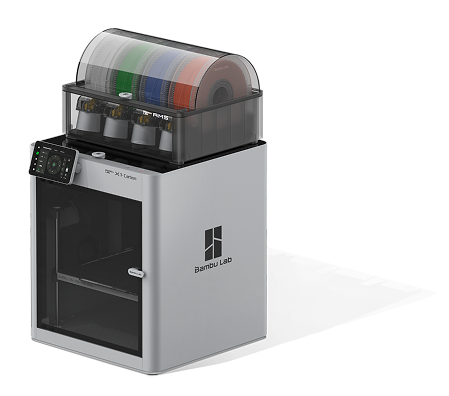
\includegraphics[width=0.8\linewidth]{Foto's/X1C}
    \caption{Bambu Lab X1C-Carbon 3D-printer. Bron: \url{https://bambulab.com/en/x1}}
    \label{fig:x1c}
\end{wrapfigure}
De Bambu Lab X1C-Carbon is een geavanceerde 3D-printer die speciaal is ontworpen voor snelheid en precisie. Enkele kenmerken zijn:
\begin{itemize}
    \item Hoge printsnelheid tot 500 mm/s
    \item CoreXY mechanisme voor stabiliteit
    \item Ondersteuning voor meerdere materialen, inclusief met koolstof versterkte filamenten
\end{itemize}
Deze printer werkt samen met de Bambu Studio slicer, een software die 3D-modellen omzet in printbare instructies \autocite{bambulabX1Carbon}.


\newpage

\section{E-commerce}%
\label{sec:E-commerce}

E-commerce is de laatste jaren uitgegroeid tot een van de belangrijkste manieren voor bedrijven om producten en diensten aan te bieden aan klanten. De opkomst van het internet en de ontwikkeling van digitale betalingssystemen hebben het gemakkelijker gemaakt voor bedrijven van elke omvang om een online winkel te starten. E-commerce omvat verschillende modellen, van B2C (Business to Consumer) tot B2B (Business to Business), en biedt tal van voordelen zoals bereikbaarheid, lage operationele kosten en de mogelijkheid om 24/7 actief te zijn~\autocite{bang2024}.

\subsection{Waarom Shopify?}

\begin{wrapfigure}{r}{0.3\textwidth}
    \centering
    
\includegraphics[width=0.8\linewidth]{Foto's/shopify-store}
    \caption{Shopify Logo. Bron: \url{https://www.ecommerce-nation.com/wp-content/uploads/2019/05/shopify-store.png.webp}}
    \label{fig:shopify-store}
\end{wrapfigure}


Shopify is een van de populairste platforms voor het bouwen van e-commerce websites. Het staat bekend om zijn gebruiksvriendelijkheid, uitgebreide functies en krachtige tools die zowel beginners als ervaren ondernemers in staat stellen om snel een online winkel te lanceren. Ook zijn er mensen rondom mij die deze tool gebruiken, zo kan er voor hen ook een 3D-printer business automatisatie geïmplementeerd worden.
\\

\subsubsection{Kenmerken van Shopify}
\begin{table}[h]
    \centering
    \begin{tabular}{|l|p{10cm}|} % 10 cm breedte voor de tweede kolom
        \hline
        \textbf{Kenmerk}            & \textbf{Beschrijving}                                                                                                                                            \\ \hline
        Gebruiksvriendelijk         & Gebruiksvriendelijke interface voor gebruikers zonder uitgebreide technische kennis.            \\ \hline
        Uitgebreide functies        & Functies zoals productbeheer, betalingsverwerking, voorraadbeheer en marketingtools.                                                \\ \hline
        Schaalbaarheid              & Geschikt voor zowel kleine als grote bedrijven, omdat het eenvoudig kan worden opgeschaald naarmate het bedrijf groeit.                                   \\ \hline
        Beveiliging                 & Shopify zorgt voor de veiligheid van klantgegevens door te voldoen aan de hoogste normen voor gegevensbeveiliging en PCI-compliantie~\autocite{bang2024}.              \\ \hline
    \end{tabular}
    \caption{Kenmerken van Shopify}
    \label{tab:shopify_features}
\end{table}

\newpage

\subsection{De Rol van Shopify in Dit Onderzoek}

In dit onderzoek wordt Shopify gebruikt om een webshop te bouwen waar specifieke producten te koop worden aangeboden. Shopify biedt de benodigde tools voor het eenvoudig beheren van producten, betalingen en klanten.

\subsubsection{De Voordelen voor Dit Project}
\begin{itemize}
     \item \textbf{Eenvoudig externe integratie:} Het is mogelijk om te gaan verbinden met een API, dit maakt het zeer handig om een pipeline aan te binden.
    \item \textbf{Eenvoudig productbeheer:} Eenvoudig om bestanden en andere digitale producten toe te voegen, beheren en verkopen via de webshop.
    \item \textbf{Betalingsverwerking:} Ondersteunt verschillende betalingsmethoden, waardoor klanten eenvoudig kunnen betalen voor hun aankopen.
    \item \textbf{Flexibiliteit en aanpasbaarheid:} De webshop kan worden aangepast aan de specifieke behoeften van het project, van het ontwerp tot de integratie van de gewenste functies~\autocite{bang2024}.
\end{itemize}

\section{API}%
\label{sec:api}

Het gebruik van API’s is ook essentieel, zo gebruiken we de \textbf{Bambu Labs-API}, die biedt een Python API voor interactie met Bambu Lab 3D Printers~\autocite{bambulabsAPI}. Er is ook de Shopify API nodig voor de bestellingen te volgen. Dat is de \textbf{Airbyte Shopify Loader} dit zorgt ervoor dat de inkomende bestellingen geladen kunnen worden~\autocite{ilamaIndexShopify}. 

\subsection{Wat is een API?}

Een API (Application Programming Interface) is een set van regels en protocollen die softwaretoepassingen in staat stelt met elkaar te communiceren. API’s fungeren als tussenpersonen tussen twee systemen, zodat ze gegevens en functionaliteit kunnen uitwisselen. API’s maken het mogelijk om interacties tussen systemen te vereenvoudigen zonder dat de gebruiker direct tussenbeide hoeft te komen.~\autocite{aws2024}.\\

API’s kunnen verschillende taken uitvoeren, van het ophalen van gegevens uit een database tot het uitvoeren van complexe berekeningen. De integratie van API’s in een systeem maakt het mogelijk om verschillende softwarecomponenten te verbinden, wat zorgt voor een robuustere en flexibele toepassing~\autocite{rapidapi2024}.

\newpage

\subsection{De mogelijkheden met de Bambu Labs-API}

\begin{itemize}
    \item Verbind en bedien Bambu Lab 3D-printers programmatisch. 
    \item Houd de printerstatus in realtime in de gaten. 
    \item Voer opdrachten uit en beheer afdruktaken via Python-code. 
    \item Eenvoudige installatie en integratie met Python\--omgevingen. 
\end{itemize}

Het kan bijvoorbeeld met het commando \texttt{bambulabs\_api.Printer.start\_print} de printer s\-tarten als  de juiste variabelen meegegeven worden~\autocite{bambulabsAPI}.Hier zit ook nog een open vraag aan voor het ophalen van het document. Dat moet nog verder onderzocht worden hoe dat in zijn werking gaat maar dat zal in de testfase gebeuren.  

\subsection{De mogelijkheden met de Shopify-API:}

\begin{itemize} 
    \item Krijg toegang tot en beheer je Shopify-bestellingen via de API. 
    \item Haal ordergegevens op, inclusief productinformatie, klantgegevens en verzendstatus. 
    \item Gebruik de Airbyte Shopify Loader om automatisch bestellingen van Shopify naar je doelbestemmingen te synchroniseren. 
\end{itemize}

Deze integratie maakt het mogelijk om bestellingen die via Shopify binnenkomen te volgen en te verwerken in een geautomatiseerde workflow. De Shopify API biedt toegang tot de ordergeschiedenis, zodat je eenvoudig kunt bijhouden welke producten zijn besteld en de status van elke bestelling kunt volgen. Het is mogelijk om orderinformatie op te halen met het commando \texttt{shopify\_api.orders.list()} om een lijst van bestellingen te verkrijgen.

\newpage

\section{Pipelines}%
\label{sec:piplines}


% Tip: Begin elk hoofdstuk met een paragraaf inleiding die beschrijft hoe
% dit hoofdstuk past binnen het geheel van de bachelorproef. Geef in het
% bijzonder aan wat de link is met het vorige en volgende hoofdstuk.

% Pas na deze inleidende paragraaf komt de eerste sectiehoofding.

%Dit hoofdstuk bevat je literatuurstudie. De inhoud gaat verder op de inleiding, maar zal het onderwerp van de bachelorproef *diepgaand* uitspitten. De bedoeling is dat de lezer na lezing van dit hoofdstuk helemaal op de hoogte is van de huidige stand van zaken (state-of-the-art) in het onderzoeksdomein. Iemand die niet vertrouwd is met het onderwerp, weet nu voldoende om de rest van het verhaal te kunnen volgen, zonder dat die er nog andere informatie moet over opzoeken \autocite{Pollefliet2011}.

%Je verwijst bij elke bewering die je doet, vakterm die je introduceert, enz.\ naar je bronnen. In \LaTeX{} kan dat met het commando \texttt{$\backslash${textcite\{\}}} of \texttt{$\backslash${autocite\{\}}}. Als argument van het commando geef je de ``sleutel'' van een ``record'' in een bibliografische databank in het Bib\LaTeX{}-formaat (een tekstbestand). Als je expliciet naar de auteur verwijst in de zin (narratieve referentie), gebruik je \texttt{$\backslash${}textcite\{\}}. Soms is de auteursnaam niet expliciet een onderdeel van de zin, dan gebruik je \texttt{$\backslash${}autocite\{\}} (referentie tussen haakjes). Dit gebruik je bv.~bij een citaat, of om in het bijschrift van een overgenomen afbeelding, broncode, tabel, enz. te verwijzen naar de bron. In de volgende paragraaf een voorbeeld van elk.

%\textcite{Knuth1998} schreef een van de standaardwerken over sorteer- en zoekalgoritmen. Experten zijn het erover eens dat cloud computing een interessante opportuniteit vormen, zowel voor gebruikers als voor dienstverleners op vlak van informatietechnologie~\autocite{Creeger2009}.

%Let er ook op: het \texttt{cite}-commando voor de punt, dus binnen de zin. Je verwijst meteen naar een bron in de eerste zin die erop gebaseerd is, dus niet pas op het einde van een paragraaf.

%\begin{figure}
  %\centering
  %
\includegraphics[width=0.8\textwidth]{grail.jpg}
  %\caption[Voorbeeld figuur.]{\label{fig:grail}Voorbeeld van invoegen van een figuur. Zorg altijd voor een uitgebreid bijschrift dat de figuur volledig beschrijft zonder in de tekst te moeten gaan zoeken. Vergeet ook je bronvermelding niet!}
%\end{figure}

%\begin{listing}
  %\begin{minted}{python}
    %import pandas as pd
   %% import seaborn as sns

    %penguins = sns.load_dataset('penguins')
   % sns.relplot(data=penguins, x="flipper_length_mm", %y="bill_length_mm", hue="species")
 % \end{minted}
  %\caption[Voorbeeld codefragment]{Voorbeeld van het invoegen van een %codefragment.}
%\end{listing}

%\lipsum[7-20]

%\begin{table}
 % \centering
 % \begin{tabular}{lcr}
   % \toprule
   % \textbf{Kolom 1} & \textbf{Kolom 2} & \textbf{Kolom 3} \\
   % $\alpha$         & $\beta$          & $\gamma$         \\
   % \midrule
   % A                & 10.230           & a                \\
   % B                & 45.678           & b                \\
    %C                & 99.987           & c                \\
   % \bottomrule
 % \end{tabular}
 % \caption[Voorbeeld tabel]{\label{tab:example}Voorbeeld van een tabel.}
%\end{table}

